\raggedbottom
\chapter{Pruebas y código}

\section{Repositorio de código}
El código fuente del proyecto \textit{BlockTrack} está alojado en el siguiente repositorio de GitHub:
\begin{itemize}
    \item \textbf{Repositorio GitHub:} \url{https://github.com/Juanjomrtz19/Trabajo-de-fin-de-grado-BlockTrack}
\end{itemize}
\section{Pruebas}
La fase de pruebas es crucial para garantizar que la aplicación \textit{BlockTrack} funcione correctamente y cumpla
con los requisitos establecidos. En este capítulo, se describen las pruebas realizadas para verificar la funcionalidad,
seguridad y rendimiento de la aplicación. En este proyecto la validación se ha centrado en pruebas unitarias para
validar flujos completos en el lado del backend y blockchain.\\

\section{Pruebas unitarias}
Las pruebas unitarias se han implementado para verificar el correcto funcionamiento de los componentes individuales
de la aplicación. El conjunto de pruebas asegura el correcto comportamiento de las funciones críticas del sistema,
en casos de error y aciertos.\\

\subsection{Tests en usuario}
Se han desarrollado pruebas unitarias con Jest para las funciones relacionadas con la gestión de usuarios, incluyendo
el registro, autenticación y actualización de perfiles. Estas pruebas verifican que los datos se manejan correctamente.

\subsubsection{POST /users/register (4 tests)}
Se han implementado 4 pruebas para el endpoint de registro de usuarios:
\begin{itemize}
    \item \textbf{Registro de enviador/receptor correctamente}: Verifica que un enviador/receptor se registre correctamente con datos válidos.
    \item \textbf{Registro de transportista exitosamente}: Comprueba que un transportista se registre correctamente con datos válidos.
    \item \textbf{Error del servicio}: Verifica manejo de errores cuando falla la base de datos durante el registro.
    \item \textbf{Comprobación de datos inválidos}: Comprueba que se retorna un error 400 si los datos de registro son inválidos.
\end{itemize}

\subsubsection{POST /users/login (3 tests)}
Se han implementado 3 pruebas para el endpoint de inicio de sesión de usuarios:
\begin{itemize}
    \item \textbf{Inicio de sesión exitoso}: Verifica que un usuario pueda iniciar sesión con credenciales válidas.
    \item \textbf{Error por credenciales inválidas}: Comprueba que se devuelva un error 401 si las credenciales son inválidas.
    \item \textbf{Usuario no encontrado}: Verifica que emails no registrados retornan un error 401.
\end{itemize}

\subsubsection{POST /users/logout (1 test)}
Se ha implementado 1 prueba para el endpoint de cierre de sesión de usuarios:
\begin{itemize}
    \item \textbf{Cierre de sesión exitoso}: Verifica que un usuario pueda cerrar sesión correctamente.
\end{itemize}

\subsubsection{GET /users/me (2 tests)}
Se han implementado 2 pruebas para el endpoint de obtención de perfil de usuario:
\begin{itemize}
    \item \textbf{Obtención de datos usuario autenticado}: Verifica que un usuario autenticado pueda obtener su perfil correctamente.
    \item \textbf{Usuario no autenticado}: Comprueba que se devuelva un error 401 si el token de autenticación es inválido o está ausente.
\end{itemize}

\subsubsection{PUT /users/updateUser (2 tests)}
Se han implementado 2 pruebas para el endpoint de actualización de perfil de usuario:
\begin{itemize}
    \item \textbf{Actualización exitosa}: Verifica que un usuario autenticado pueda actualizar su perfil correctamente.
    \item \textbf{Error en actualización}: Comprueba que se devuelva un error 500 si ocurre un problema durante la actualización del perfil.
\end{itemize}

\subsubsection{Resultados tests usuario}
En total se han implementado 12 pruebas unitarias para la gestión de usuarios, todas las cuales han sido exitosas,
lo que garantiza la robustez y fiabilidad de esta funcionalidad crítica en la aplicación.
\begin{figure}
    \centering
    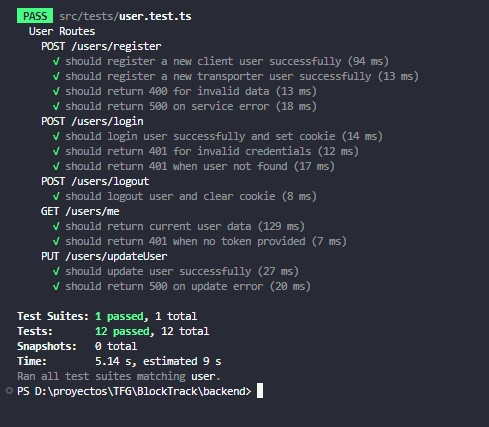
\includegraphics[width=0.8\textwidth]{imagenes/Pruebas/testUsers.jpg}
    \caption{Resultados de las pruebas unitarias para la gestión de usuarios}
\end{figure} 

\subsection{Tests en remesa}
Se han desarrollado pruebas unitarias con Jest para las funciones relacionadas con la gestión de remesas.
\subsubsection{POST /remesas (3 tests)}
Se han implementado 3 pruebas para el endpoint de creación de remesas:
\begin{itemize}
    \item \textbf{Creación de remesa correctamente}: Verifica que una remesa se cree correctamente con datos válidos.
    \item \textbf{Usuario no es enviador/receptor}: Verifica que se retorna un error 403 si el usuario no tiene ese rol en la aplicación, en resumen, si el usuario
es transportista no debe poder crear remesas.
    \item \textbf{Comprobación de datos inválidos}: Comprueba que se retorna un error 400 si los datos de creación son inválidos.
\end{itemize}

\subsubsection{GET /remesas (1 tests)}
Se ha implementado 1 prueba para el endpoint de obtención de remesas:
\begin{itemize}
    \item \textbf{Obtención de remesas correctamente}: Verifica que se devuelven las remesas del usuario autenticado.
\end{itemize}

\subsubsection{GET /remesas/:idRemesa (2 tests)}
Se han implementado 2 pruebas para el endpoint de obtención de una remesa específica:
\begin{itemize}
    \item \textbf{Obtención de remesa correctamente}: Verifica que se devuelve la remesa solicitada si existe.
    \item \textbf{ID inválido}: Comprueba que Ids no numéricos retornan un error 400.
\end{itemize}

\subsubsection{PUT /remesas/:idRemesa (2 tests)}
Se han implementado 2 pruebas para el endpoint de actualización de una remesa específica:
\begin{itemize}
    \item \textbf{Actualización de remesa correctamente}: Verifica que una remesa se actualice correctamente con datos válidos.
    \item \textbf{Datos de actualización inválidos}: Verifica que se retorna un error 400 si los datos de actualización son inválidos.
\end{itemize}

\subsubsection{PATCH /remesas/cancelarRemesa/:idRemesa (2 tests)}
Se han implementado 2 pruebas para el endpoint de cancelación de una remesa específica:
\begin{itemize}
    \item \textbf{Cancelación de remesa correctamente}: Verifica que una remesa se cancele correctamente si el usuario es el enviador.
    \item \textbf{Error al cancelar}: Comprueba manejo de errores cuando no se puede cancelar la remesa.
\end{itemize}

\subsubsection{POST /remesas/asignarTransportistas/:idRemesa (2 tests)}
Se han implementado 2 pruebas para el endpoint de asignación de transportistas a una remesa específica:

\begin{itemize}
    \item \textbf{Asignación de transportistas correctamente}: Verifica que los transportistas se asignen correctamente a la remesa.
    \item \textbf{Error al asignar transportistas}: Comprueba manejo de errores cuando no se pueden asignar transportistas.
\end{itemize}

\subsubsection{Resultados tests remesa}
En total se han implementado 12 pruebas unitarias para la gestión de remesas, todas las cuales han sido exitosas,
lo que garantiza la robustez y fiabilidad de esta funcionalidad crítica en la aplicación.

\begin{figure}
    \centering
    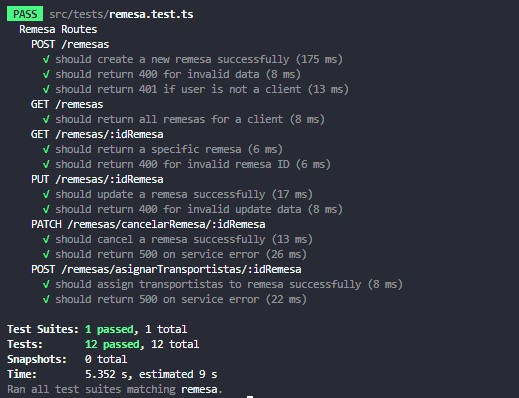
\includegraphics[width=0.8\textwidth]{imagenes/Pruebas/testRemesas.jpg}
    \caption{Resultados de las pruebas unitarias para la gestión de remesas}
\end{figure}

\subsection{Tests en transporte}
Se han desarrollado pruebas unitarias con jest para las funciones relacionadas con la gestión de transportes.
\subsubsection{POST /transportes (3 tests)}
Se han implementado 3 pruebas para el endpoint de creación de transportes:
\begin{itemize}
    \item \textbf{Creación de transporte correctamente}: Verifica que un transporte se cree correctamente con datos válidos.
    \item \textbf{Usuario no es transportista}: Verifica que se retorna un error 401 si el usuario no tiene ese rol en la aplicación, en resumen, si el usuario
    \item \textbf{Comprobación de datos inválidos}: Comprueba que se retorna un error 500 si los datos de creación son inválidos.
\end{itemize}

\subsubsection{GET /transportes (1 test)}
Se ha implementado 1 prueba para el endpoint de obtención de transportes:
\begin{itemize}
    \item \textbf{Obtención de transportes correctamente}: Verifica que se devuelven los transportes del transportista autenticado.
\end{itemize}

\subsubsection{PUT /transportes/:id (2 tests)}
Se han implementado 2 pruebas para el endpoint de actualización de un transporte específico:
\begin{itemize}
    \item \textbf{Actualización de transporte correctamente}: Verifica que un transporte se actualice correctamente con datos válidos.
    \item \textbf{Datos de actualización inválidos}: Verifica que se retorna un error 500 si los datos de actualización son inválidos.
\end{itemize}

\subsubsection{DELETE /transportes/:id (1 test)}
Se ha implementado 1 prueba para el endpoint de eliminación de un transporte específico:
\begin{itemize}
    \item \textbf{Eliminación de transporte correctamente}: Verifica que un transporte se elimine correctamente si existe.
\end{itemize}

\subsubsection{Resultados tests transporte}
En total se han implementado 7 pruebas unitarias para la gestión de transportes, todas las cuales han sido exitosas.
\begin{figure}
    \centering
    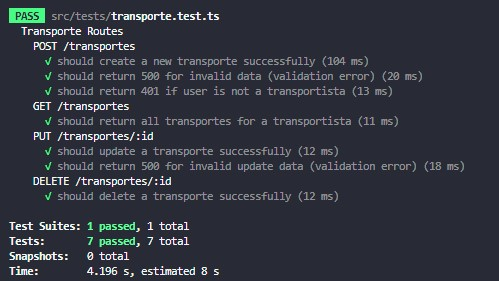
\includegraphics[width=0.8\textwidth]{imagenes/Pruebas/testTransporte.jpg}
    \caption{Resultados de las pruebas unitarias para la gestión de transportes}
\end{figure}

\section{Pruebas de contratos inteligentes}
Las pruebas de los contratos inteligentes son fundamentales para garantizar la seguridad y funcionalidad de la lógica
implementada en la blockchain. Se han desarrollado pruebas específicas para cada función del contrato inteligente
\texttt{EnvioFactory} y \texttt{Envio}.\\

Además en el ámbito de la tecnología blockchain, esta fase cobra vital importancia ya que una vez los contratos estén desplegados
en la red, no se pueden modificar. Por ello, se han realizado pruebas exhaustivas para asegurar que los contratos
funcionan correctamente.\\

\subsection{Contrato Envio}
En el caso del contrato Envio se han realizado un gran número de pruebas entre la que destacan:
\begin{itemize}
    \item \textbf{Creación de envíos}: Verificar que un nuevo envío se crea correctamente con los parámetros adecuados.
    \item \textbf{Actualización de estado}: Asegurar que los estados del envío se actualizan correctamente en función de las acciones realizadas por los usuarios.
    \item \textbf{Añadir transportistas aceptados}: Comprobar que los transportistas pueden ser añadidos correctamente a un envío.
    \item \textbf{Cambio del poseedor}: Validar que el poseedor del envío se actualiza correctamente.
    \item \textbf{Casos de error}: Probar que las funciones manejan adecuadamente los casos de error, como intentos no autorizados de actualizar el estado del envío o
    añadir transportistas aceptados cuando la cantidad de transportistas aceptados ya es igual al número máximo permitido.
\end{itemize}



\subsection{Contrato EnvioFactory}
En el caso del contrato EnvioFactory se han realizado pruebas para:
\begin{itemize}
    \item \textbf{Creación de envíos}: Verificar que un nuevo envío se crea correctamente y se almacena en el mapeo de envíos.
    \item \textbf{Recuperación de envíos}: Asegurar que los envíos pueden ser recuperados correctamente utilizando su ID.
    \item \textbf{Casos de error}: Probar que las funciones manejan adecuadamente los casos de error, como intentos de recuperar un envío inexistente.
\end{itemize}

\subsection{Resultado de las pruebas}
En el estado actual del sistema, todas las pruebas implementadas han sido exitosas, lo que proporciona
una alta confianza en la funcionalidad y seguridad de la aplicación \textit{BlockTrack} y debido al ciclo iterativo de
la metodología ágil, según se encontraron nuevos errores o fallos, se iban añadiendo mejoras y nuevas pruebas para
garantizar la calidad del software.
\begin{figure}
    \centering
    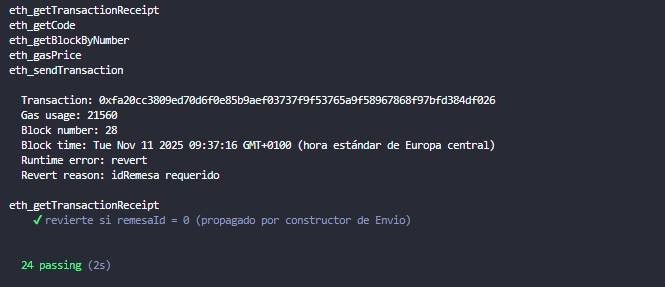
\includegraphics[width=0.8\textwidth]{imagenes/Pruebas/resultadoTestSmartContracts.jpg}
    \caption{Resultados de las pruebas unitarias para los contratos inteligentes}
\end{figure}

\section{Conclusión de la fase de pruebas}
La fase de pruebas ha sido esencial para validar la funcionalidad, seguridad y rendimiento de la aplicación
\textit{BlockTrack}. El backend y contratos inteligentes han sido rigurosamente probados mediante pruebas, asegurando
que cumplen con los requisitos establecidos y funcionan correctamente en diversos escenarios. Los resultados positivos
de las pruebas proporcionan una base sólida para la implementación y despliegue de la aplicación en un entorno real.